\clearpage % Rozdziały zaczynamy od nowej strony.
\section{Techniki tworzenia skalowalnych aplikacji webowych}

Taki rozdział w ogóle będzie przydatny?

\subsection{Architektura mikroserwisowa}

Architektura mikroserwisowa to podejście do strukturyzacji aplikacji jako zbiór niewielkich, niezależnych usług, które komunikują się ze sobą przy użyciu standardowych protokołów komunikacji synchronicznej, takich jak HTTP/gRPC \cite{grpc} lub asynchronicznych kolejek komunikatów, np. RabbitMQ \cite{rabbitmq}/Apache Kafka \cite{kafka}. Każdy mikroserwis jest odpowiedzialny za wykonanie określonej funkcjonalności lub usługi i może być rozwijany, wdrażany oraz zarządzany niezależnie od innych. Ta architektura zapewnia wysoką skalowalność i elastyczność, umożliwiając łatwe wprowadzanie zmian i adaptację do zmieniających się wymagań. Mikroserwisy przechowujące dane często mają swoje własne bazy danych, co zwiększa ich niezależność i izolację od innych części systemu.

\begin{figure}[!h]
    \centering 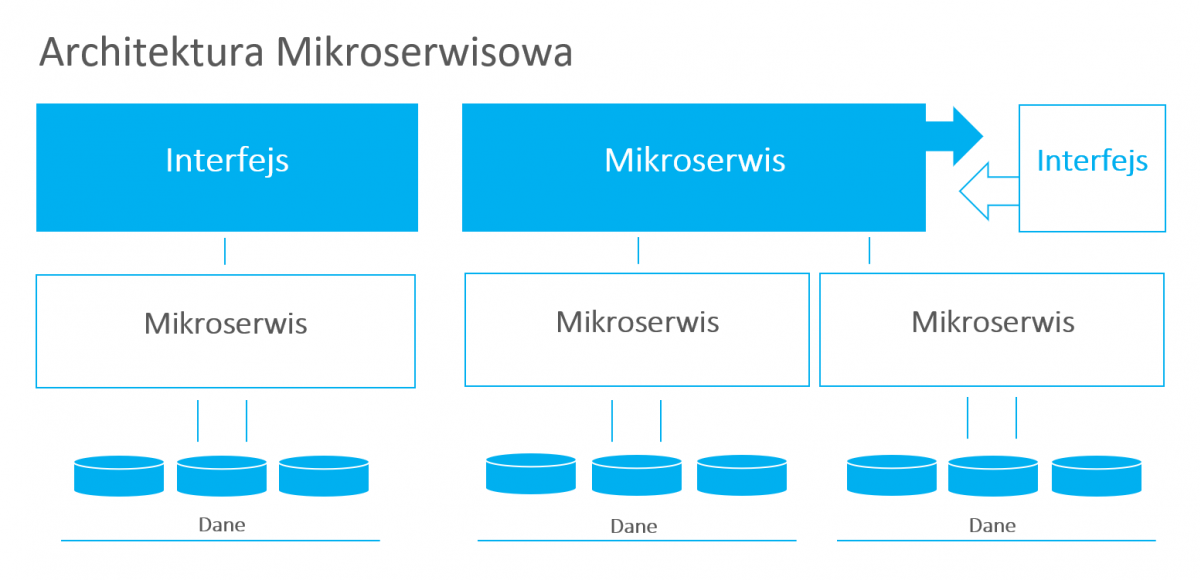
\includegraphics[width=1.0\linewidth]{mikroserwisy.png}
    \caption{Reprezentacja graficzna systemu o architekturze mikroserwisowej \cite{rys1}}
\end{figure}


Główną konsekwencją zastosowania takiej architektury, jest możliwości niezależnego poziomego skalowania każdego komponentu systemu, ponieważ każdy serwis jest osobną jednostką wdrożeniową (np. kontenerem).

Z powodu konieczności komunikacji między elementami systemu, często utrudnione jest zastosowanie spójności natychmiastowej, znanej np. z relacyjnych baz danych. W systemach takich stosowana jest tzw. spójność ostateczna (ang. "eventual consistency") \cite{eventual_consistency}. Powoduje ona, że najnowszy odczyt nie gwarantuje otrzymania danych wynikających z najnowszego zapisu. Utrudnia to m.in. tworzenie interfejsów graficznych dla użytkowników końcowych oraz testowanie aplikacji.

Stosując architekturę mikroserwisową, systemy informatyczne mogą spełniać wymagania dotyczące wysokiej niezawodności i dostępności - każdy serwis może być uruchomiony w więcej niż jednej instancji, równo rozkładając ruch pomiędzy nie. System jest wtedy też odporny na chwilową niedostępność niektórych instancji.

TODO porównanie z monolitem

\subsection{Skalowalność}

Skalowanie usług jest ważnym aspektem w projektowaniu i utrzymaniu aplikacji internetowych, zwłaszcza w kontekście rosnącego zapotrzebowania na usługi danej aplikacji, spowodowanego np. wzrostem liczby użytkowników. W kontekście systemów informatycznych, skalowanie może być realizowane zarówno w sposób poziomy, jak i pionowy.

Skalowanie Poziome: Oznacza dodawanie większej liczby instancji serwisu do obsługi rosnącego obciążenia. W przypadku mikroserwisów, indywidualne serwisy mogą być skalowane niezależnie, co pozwala na zwiększenie wydajności systemu bez konieczności modyfikowania całej architektury. W rozwiązaniach chmurowych takie skalowanie jest bardzo często automatyczne - odpowiednie mechanizmy uruchamiają kolejne instancje serwisów na podstawie zużycia ich zasobów lub np. liczby żądań na sekundę.

Skalowanie Pionowe: Polega na zwiększaniu zasobów (np. CPU, pamięci) w istniejącej instancji serwisu. W architekturze mikroserwisowej jest to mniej powszechne, ponieważ główny nacisk kładzie się na elastyczność i skalowalność poziomą. Skalowanie takie jest bardzo popularne w systemach o architekturze monolitycznej, ponieważ często jest to jedyna opcja na zwiększenie wydajności rozwiązania bez poważnych zmian w architekturze.

Architektura mikroserwisowa umożliwia efektywne skalowanie dzięki izolacji poszczególnych serwisów, co umożliwia ich niezależne zarządzanie, rozwój i skalowanie w zależności od indywidualnych potrzeb i zapotrzebowania. Dzięki temu możliwe jest efektywne zarządzanie zasobami i optymalizacja wydajności systemu.

Tworząc rozproszone systemy przetwarzające dane, należy pamiętać o tzw. twierdzeniu Brewera o CAP.

\begin{figure}[!h]
    \centering 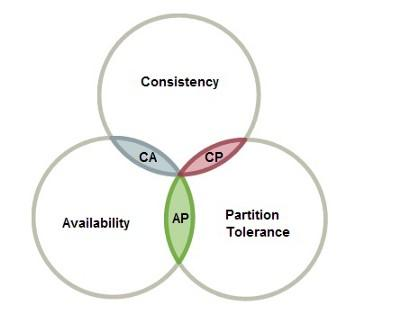
\includegraphics[width=0.5\linewidth]{cap.jpg}
    \caption{Reprezentacja graficzna twierdzenia CAP \cite{rys2}}
\end{figure}

Twierdzenie CAP, odnosi się do trzech podstawowych właściwości, które mogą być gwarantowane w systemach rozproszonych: spójność (Consistency), dostępność (Availability) oraz odporność na rozbicia (Partition Tolerance). Stwierdza ono, że system rozproszony może zapewnić jednocześnie tylko dwie z tych trzech właściwości. Decyzje dotyczące skalowania i zarządzania danymi muszą uwzględniać kompromisy między spójnością, dostępnością i odpornością na rozbicia.

TODO

\subsection{Architektura zorientowana na zdarzenia}

XXX

\subsection{Projektowanie zorientowane na dziedzinę}

Domain-Driven Design (DDD) to podejście do projektowania oprogramowania skoncentrowane na modelowaniu i strukturyzacji systemów zgodnie z realiami i złożonościami określonej dziedziny biznesowej. W DDD kluczowe jest głębokie zrozumienie dziedziny i jej problemów, co umożliwia tworzenie efektywnych modeli i struktur aplikacji. W kontekście tworzenia skalowalnych aplikacji webowych, DDD pomaga w wyodrębnieniu granic kontekstów, co jest szczególnie istotne w architekturze mikroserwisowej. Pozwala to na efektywne projektowanie niezależnych mikroserwisów, każdy z nich odpowiedzialny za różne aspekty dziedziny biznesowej, co przyczynia się do lepszej skalowalności i łatwości w zarządzaniu.

TODO

\subsection{Separacja odpowiedzialności komend i zapytań}

Command Query Responsibility Segregation (CQRS) to wzorzec projektowy, który rozdziela operacje odczytu (Query) od operacji zapisu (Command) w systemie informatycznym. W kontekście tworzenia skalowalnych aplikacji webowych, CQRS umożliwia niezależne skalowanie i optymalizację operacji odczytu i zapisu. Pozwala to na efektywniejsze wykorzystanie zasobów, zmniejsza złożoność kodu i zwiększa wydajność aplikacji. CQRS jest często stosowany w architekturze mikroserwisowej, gdzie może dodatkowo przyczynić się do lepszej separacji odpowiedzialności pomiędzy różnymi mikroserwisami.

\begin{figure}[!h]
    \centering 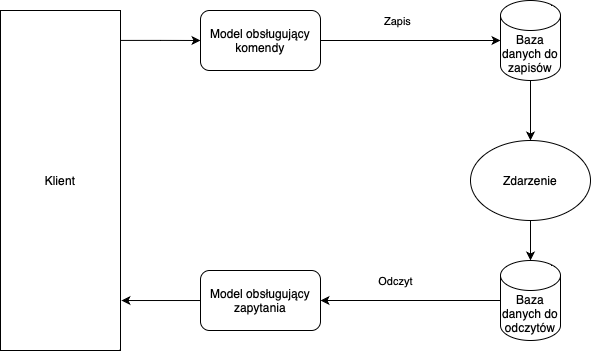
\includegraphics[width=0.6\linewidth]{cqrs.png}
    \caption{Schemat architektoniczny implementacji wzorca CQRS}
\end{figure}

TODO

\subsection{Event Sourcing}

Event Sourcing to podejście w projektowaniu oprogramowania, w którym zmiany stanu aplikacji są przechowywane jako sekwencja zdarzeń. Zamiast zapisywać tylko bieżący stan obiektu, system zachowuje pełną historię zmian za pomocą zdarzeń, które te zmiany spowodowały. W kontekście tworzenia skalowalnych aplikacji webowych, Event Sourcing umożliwia efektywne zarządzanie i rekonstruowanie stanów systemu, zapewniając wysoce odporną na błędy i elastyczną architekturę. Ta metoda jest szczególnie przydatna w środowiskach rozproszonych, takich jak architektura mikroserwisowa, gdzie zachowanie spójności i odporności na awarie jest pożądane.

\begin{figure}[!h]
    \centering 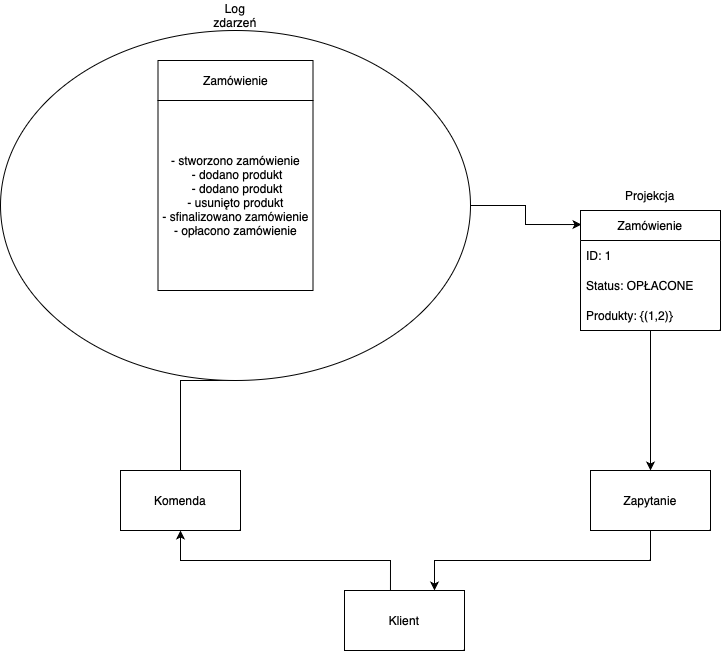
\includegraphics[width=0.8\linewidth]{event_sourcing.png}
    \caption{Schemat architektoniczny implementacji wzorca Event Sourcing}
\end{figure}

TODO

\subsection{Wzorzec Saga}

Wzorzec Saga w projektowaniu oprogramowania odnosi się do sekwencyjnego lub równoległego wykonywania serii operacji w rozproszonym systemie, takim jak architektura mikroserwisowa. W kontekście skalowalnych aplikacji webowych, Saga zapewnia spójne zarządzanie transakcjami rozproszonymi poprzez rozkładanie ich na serię mniejszych, zarządzalnych operacji. Każda operacja w ramach Sagii jest wykonywana niezależnie, a w przypadku wystąpienia błędu, system może wykonać odpowiednie operacje kompensujące, aby przywrócić spójność danych. Wzorzec ten jest istotny w zarządzaniu złożonymi transakcjami w skalowalnych i rozproszonych systemach, gdzie tradycyjne transakcje bazodanowe mogą być niewystarczające.

TODO